% Beamer version of the presentation. Self-contained: every chart is drawn
% with pgfplots from the measurements in results/ (see slides/data.json), so
% the file can be pasted into Overleaf without uploading any figures.
% Compile with pdfLaTeX.
\documentclass[aspectratio=169,11pt]{beamer}

\usetheme{default}
\usefonttheme{professionalfonts}
\setbeamertemplate{navigation symbols}{}
\setbeamertemplate{footline}{%
  \hfill\usebeamercolor[fg]{footline}\scriptsize
  Finite field determinants \quad\textperiodcentered\quad CSE 625
  \quad\insertframenumber/\inserttotalframenumber\hspace*{1em}\vspace*{0.6em}}

\usepackage[T1]{fontenc}
\usepackage{lmodern}
\usepackage{booktabs}
\usepackage{array}
\usepackage{tikz}
\usetikzlibrary{arrows.meta,positioning,shapes.geometric}
\usepackage{pgfplots}
\pgfplotsset{compat=1.17}

% Colours
\definecolor{ink}{HTML}{1F2937}
\definecolor{muted}{HTML}{6B7280}
\definecolor{accent}{HTML}{AD0000}   % Louisville red
\definecolor{original}{HTML}{9CA3AF}
\definecolor{cached}{HTML}{2563EB}
\definecolor{mapcol}{HTML}{F59E0B}
\definecolor{ptwo}{HTML}{10B981}
\definecolor{pfour}{HTML}{7C3AED}

\setbeamercolor{normal text}{fg=ink}
\setbeamercolor{frametitle}{fg=accent}
\setbeamercolor{title}{fg=accent}
\setbeamercolor{structure}{fg=accent}
\setbeamercolor{footline}{fg=muted}
\setbeamerfont{frametitle}{series=\bfseries,size=\Large}
\setbeamertemplate{itemize items}[circle]

\pgfplotsset{
  every axis/.append style={
    font=\footnotesize,
    axis lines*=left,
    grid=major,
    grid style={gray!20},
    legend style={draw=none,fill=none,font=\footnotesize},
    legend cell align=left,
  },
}

\newcommand{\stat}[2]{%
  \begin{minipage}[t]{\linewidth}\centering
    {\Huge\bfseries\color{accent}#1}\\[0.3em]
    {\small\color{muted}#2}
  \end{minipage}}

\title{Caching Finite Field Arithmetic and\\Distributing Determinants with MPI}
\author{Group 3}
\institute{CSE 625 Parallel Programming\\University of Louisville}
\date{}

\begin{document}

% ---------------------------------------------------------------------------
\begin{frame}[plain]
  \titlepage
\end{frame}

% ---------------------------------------------------------------------------
\begin{frame}{The problem}
  \begin{columns}[T]
    \begin{column}{0.58\textwidth}
      \begin{itemize}
        \item Compute $C = A \times B$, then $\det A$, $\det B$, $\det C$ independently
              and check $\det C = \det A \cdot \det B$.
        \item Entries live in $\mathrm{GF}(11^3)$: \textbf{1331} elements.
        \item Each element is a polynomial of degree $< 3$ with coefficients mod 11,
              so every add and multiply is polynomial arithmetic plus a reduction.
        \item Only 1331 values exist, so the \emph{same} operations repeat
              billions of times.
      \end{itemize}
    \end{column}
    \begin{column}{0.38\textwidth}
      \vspace{0.5em}
      \stat{$3.2\times10^{11}$}{field operations at $N=4000$\\(product $\approx 2N^3$, three determinants $\approx N^3$)}
      \\[1.5em]
      \stat{$1331^2 = 1\,771\,561$}{distinct operand pairs}
    \end{column}
  \end{columns}
\end{frame}

% ---------------------------------------------------------------------------
\begin{frame}{Where the finite field sits in the dependency chain}
  \centering
  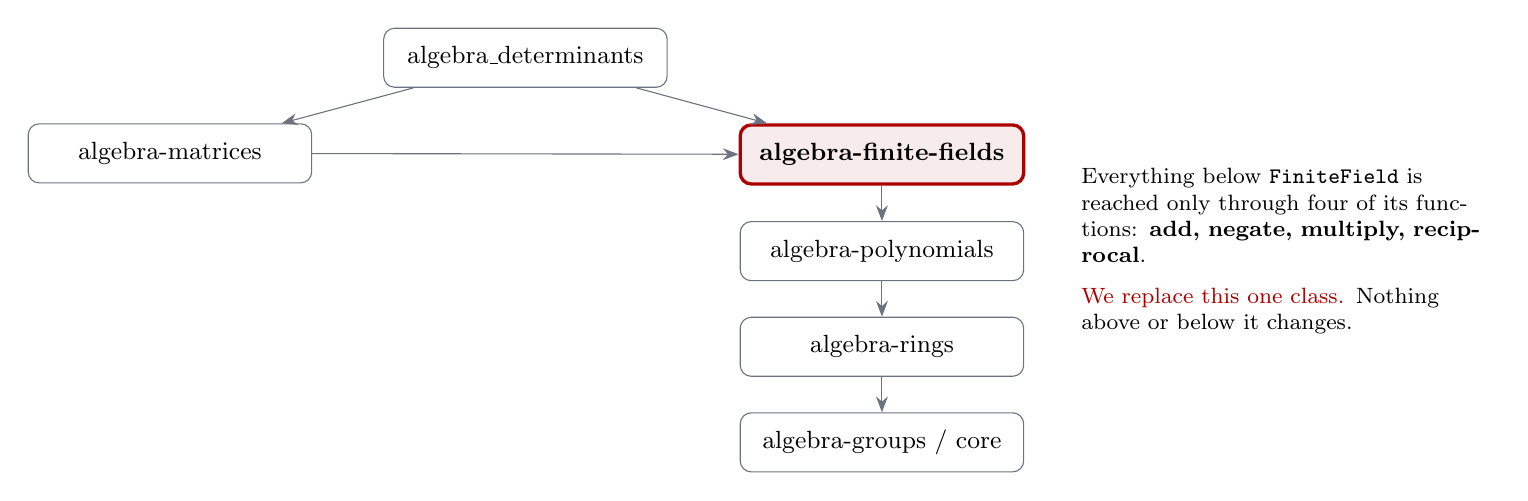
\begin{tikzpicture}[
      node distance=0.45cm and 0.9cm,
      lib/.style={draw=muted,rounded corners,minimum width=3.6cm,minimum height=0.75cm,
                  font=\small,fill=white},
      hot/.style={lib,draw=accent,very thick,fill=accent!8,font=\small\bfseries},
      dep/.style={-{Stealth[length=2mm]},muted}]
    \node[lib]  (prog)  {algebra\_determinants};
    \node[lib,  below left=of prog]  (mat) {algebra-matrices};
    \node[hot,  below right=of prog] (ff)  {algebra-finite-fields};
    \node[lib,  below=of ff]  (poly) {algebra-polynomials};
    \node[lib,  below=of poly] (ring) {algebra-rings};
    \node[lib,  below=of ring] (grp)  {algebra-groups / core};
    \draw[dep] (prog) -- (mat);
    \draw[dep] (prog) -- (ff);
    \draw[dep] (mat)  -- (ff);
    \draw[dep] (ff)   -- (poly);
    \draw[dep] (poly) -- (ring);
    \draw[dep] (ring) -- (grp);
    \node[right=0.6cm of poly,align=left,font=\footnotesize,text width=5.2cm] {%
      Everything below \texttt{FiniteField} is reached only through four of its
      functions: \textbf{add, negate, multiply, reciprocal}.\\[0.6em]
      \textcolor{accent}{We replace this one class.} Nothing above or below it changes.};
  \end{tikzpicture}
\end{frame}

% ---------------------------------------------------------------------------
\begin{frame}{Profiling: the arithmetic is the target}
  \begin{columns}[c]
    \begin{column}{0.62\textwidth}
      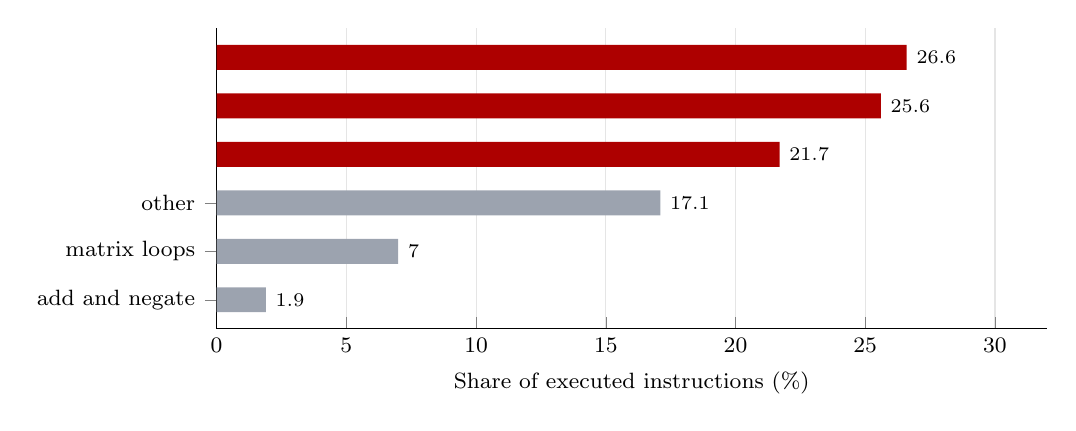
\begin{tikzpicture}
        \begin{axis}[
            xbar, width=\linewidth, height=5.4cm,
            xmin=0, xmax=32,
            xlabel={Share of executed instructions (\%)},
            symbolic y coords={{add and negate},{matrix loops},{other},{heap allocation},{multiplication},{reduction (divmod)}},
            ytick=data, y dir=normal,
            yticklabel style={font=\footnotesize},
            nodes near coords, nodes near coords style={font=\scriptsize},
            bar width=9pt, bar shift=0pt, ymajorgrids=false, enlarge y limits=0.12]
          \addplot[fill=original,draw=none] coordinates {
            (1.9,{add and negate}) (7.0,{matrix loops}) (17.1,{other})};
          \addplot[fill=accent,draw=none] coordinates {
            (21.7,{heap allocation}) (25.6,{multiplication}) (26.6,{reduction (divmod)})};
        \end{axis}
      \end{tikzpicture}
    \end{column}
    \begin{column}{0.35\textwidth}
      \stat{76\,\%}{of instructions are polynomial arithmetic and the allocations it causes}
      \\[1.2em]
      \stat{7\,\%}{is the matrix loops themselves}
      \\[1em]
      {\scriptsize\color{muted}Callgrind, original program, $N=60$.}
    \end{column}
  \end{columns}
\end{frame}

% ---------------------------------------------------------------------------
\begin{frame}{The cached field: an operation becomes one table read}
  \begin{columns}[T]
    \begin{column}{0.5\textwidth}
      \begin{itemize}
        \item A cached element stores only its \textbf{index} $0\ldots1330$
              (the base-11 digits of its coefficients): 2 bytes.
        \item Dense tables of $1331^2$ slots for $+$ and $\times$,
              1331 slots for negation and reciprocal.
        \item Slots start empty and fill \textbf{lazily}.
        \item Miss $\Rightarrow$ call the \textbf{original} \texttt{FiniteField} arithmetic,
              store the result.
        \item Irreducible polynomial: taken from the original class's deterministic search.
      \end{itemize}
    \end{column}
    \begin{column}{0.48\textwidth}
      \centering
      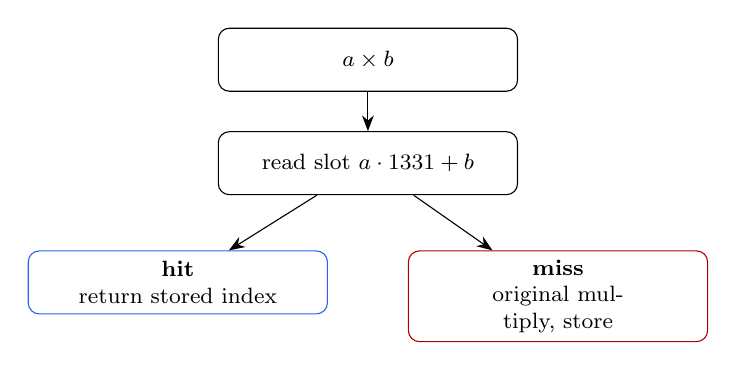
\begin{tikzpicture}[
          box/.style={draw,rounded corners,align=center,font=\footnotesize,
                      minimum width=3.8cm,minimum height=0.8cm},
          arr/.style={-{Stealth[length=2mm]}}]
        \node[box] (in) {$a \times b$};
        \node[box,below=0.5cm of in] (read) {read slot $a\cdot1331+b$};
        \node[box,below left=0.7cm and -1.4cm of read,draw=cached,text width=2.6cm] (hit)
             {\textbf{hit}\\return stored index};
        \node[box,below right=0.7cm and -1.4cm of read,draw=accent,text width=2.6cm] (miss)
             {\textbf{miss}\\original multiply, store};
        \draw[arr] (in) -- (read);
        \draw[arr] (read) -- (hit);
        \draw[arr] (read) -- (miss);
      \end{tikzpicture}\\[0.8em]
      {\footnotesize Slots are relaxed atomics: every thread that fills a slot
       writes the same value, so it is thread-safe without locks.}
    \end{column}
  \end{columns}
\end{frame}

% ---------------------------------------------------------------------------
\begin{frame}{Why a table and not \texttt{std::unordered\_map}}
  \begin{columns}[c]
    \begin{column}{0.62\textwidth}
      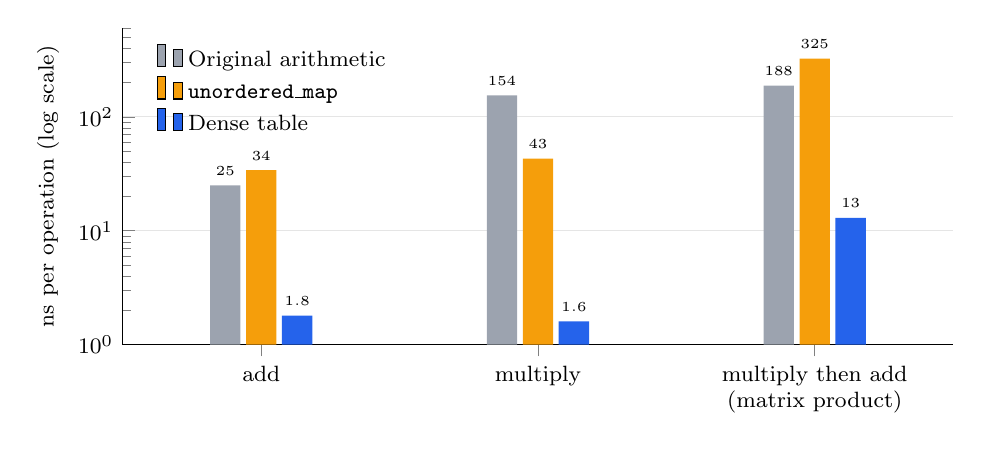
\begin{tikzpicture}
        \begin{axis}[
            ybar, width=\linewidth, height=5.6cm,
            ymode=log, log origin=infty, ymin=1, ymax=600,
            ylabel={ns per operation (log scale)},
            symbolic x coords={add,multiply,chained},
            xticklabels={add,multiply,{multiply then add\\(matrix product)}},
            xticklabel style={align=center},
            xtick=data, bar width=11pt, enlarge x limits=0.25,
            legend pos=north west, xmajorgrids=false,
            nodes near coords, nodes near coords style={font=\tiny},
            point meta=rawy]
          \addplot[fill=original,draw=none] coordinates {(add,25) (multiply,154) (chained,188)};
          \addplot[fill=mapcol,draw=none]   coordinates {(add,34) (multiply,43)  (chained,325)};
          \addplot[fill=cached,draw=none]   coordinates {(add,1.8) (multiply,1.6) (chained,13)};
          \legend{Original arithmetic, \texttt{unordered\_map}, Dense table}
        \end{axis}
      \end{tikzpicture}
    \end{column}
    \begin{column}{0.35\textwidth}
      \begin{itemize}
        \item In the chained pattern of the matrix product the hash map is
              \textbf{slower than the original} (325 vs.\ 188 ns).
        \item The table is \textbf{14.5$\times$} faster than the original there.
        \item The key space is tiny and dense: hashing buys nothing.
      \end{itemize}
    \end{column}
  \end{columns}
\end{frame}

% ---------------------------------------------------------------------------
\begin{frame}[fragile]{A drop-in replacement: one CMake entry}
  \begin{columns}[T]
    \begin{column}{0.55\textwidth}
      \small\texttt{cmake/Dependencies.cmake}
\begin{semiverbatim}\footnotesize
FetchContent_Declare(
    algebra_finite_fields
    GIT_REPOSITORY \textcolor{accent}{\textbf{git@github.com:Jplangdon/}}
      \textcolor{accent}{\textbf{algebra-finite-fields-cached.git}}
    GIT_TAG        \textcolor{accent}{\textbf{cached-v1}}
)
\end{semiverbatim}
      \vspace{0.3em}
      {\footnotesize Point it back at the original repository and the
      original program builds unchanged.}
    \end{column}
    \begin{column}{0.42\textwidth}
      \textbf{Preserved}
      \begin{itemize}\small
        \item class and type names: \texttt{algebra::FiniteField},
              \texttt{FiniteFieldElement}
        \item header paths and the CMake target \texttt{algebra::finite\_fields}
        \item every public method signature
      \end{itemize}
      \textbf{Added only}
      \begin{itemize}\small
        \item \texttt{uncached\_type}, \texttt{is\_cached}, \texttt{cache\_statistics()}
      \end{itemize}
      \texttt{src/main.cpp} is untouched.
    \end{column}
  \end{columns}
\end{frame}

% ---------------------------------------------------------------------------
\begin{frame}{Same results: checked against the original}
  \begin{columns}[T]
    \begin{column}{0.5\textwidth}
      \textbf{Unit tests (GoogleTest)}
      \begin{itemize}\small
        \item $+$ and $\times$ on \textbf{all 1\,771\,561 pairs}, once while filling
              the tables and again from the tables
        \item negation and reciprocal on all 1331 elements;
              reciprocal of zero still throws
        \item subtraction, division and compound operators on random pairs
        \item $40\times40$ determinants, several threads, a field too large to cache
      \end{itemize}
    \end{column}
    \begin{column}{0.46\textwidth}
      \textbf{Whole program}
      \begin{itemize}\small
        \item Original and cached print \textbf{identical} determinants
              at $N = 100, 200, 400, 800, 1000$.
        \item $\det C = \det A\cdot\det B$ holds in every run.
      \end{itemize}
      \vspace{0.5em}
      {\footnotesize\color{muted}The original library's own tests are also run, unchanged,
       against the cached build.}
    \end{column}
  \end{columns}
\end{frame}

% ---------------------------------------------------------------------------
\begin{frame}{Run time before and after caching}
  \begin{columns}[c]
    \begin{column}{0.6\textwidth}
      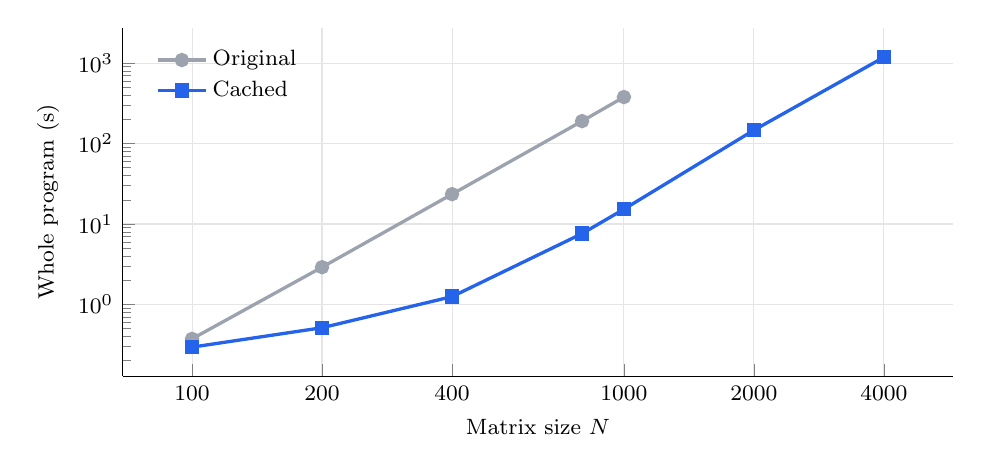
\begin{tikzpicture}
        \begin{axis}[
            width=\linewidth, height=6cm,
            xmode=log, ymode=log, log basis x=10,
            xlabel={Matrix size $N$}, ylabel={Whole program (s)},
            xtick={100,200,400,1000,2000,4000},
            xticklabels={100,200,400,1000,2000,4000},
            legend pos=north west]
          \addplot[original,very thick,mark=*] coordinates {
            (100,0.374) (200,2.906) (400,23.485) (800,189.932) (1000,378.109)};
          \addplot[cached,very thick,mark=square*] coordinates {
            (100,0.295) (200,0.514) (400,1.252) (800,7.597) (1000,15.282)
            (2000,146.576) (4000,1182.199)};
          \legend{Original, Cached}
        \end{axis}
      \end{tikzpicture}
    \end{column}
    \begin{column}{0.37\textwidth}
      \stat{24.7$\times$}{faster at $N=1000$\\6 min 18 s $\rightarrow$ 15.3 s}
      \\[1em]
      \stat{19 min 42 s}{cached, $N=4000$}
      \\[0.6em]
      {\scriptsize\color{muted}Assignment reference (M3 Max): 6 h 40 min original,
       20 min 16 s cached. Our original was not run at 4000; an $N^3$
       extrapolation gives $\approx$ 6 h 43 min.}
    \end{column}
  \end{columns}
\end{frame}

% ---------------------------------------------------------------------------
\begin{frame}{Small matrices gain little: the tables fill first}
  \begin{columns}[c]
    \begin{column}{0.49\textwidth}
      \centering{\small Speedup of the whole program}\\
      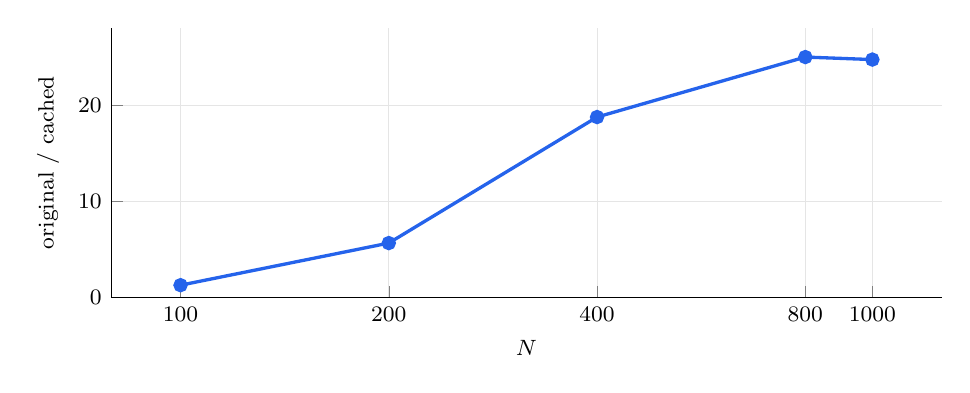
\begin{tikzpicture}
        \begin{axis}[
            width=\linewidth, height=5cm, xmode=log,
            xlabel={$N$}, ylabel={original / cached},
            xtick={100,200,400,800,1000}, xticklabels={100,200,400,800,1000},
            ymin=0, ymax=28]
          \addplot[cached,very thick,mark=*] coordinates {
            (100,1.27) (200,5.65) (400,18.76) (800,25.00) (1000,24.74)};
        \end{axis}
      \end{tikzpicture}
    \end{column}
    \begin{column}{0.49\textwidth}
      \centering{\small Operations answered from a table}\\
      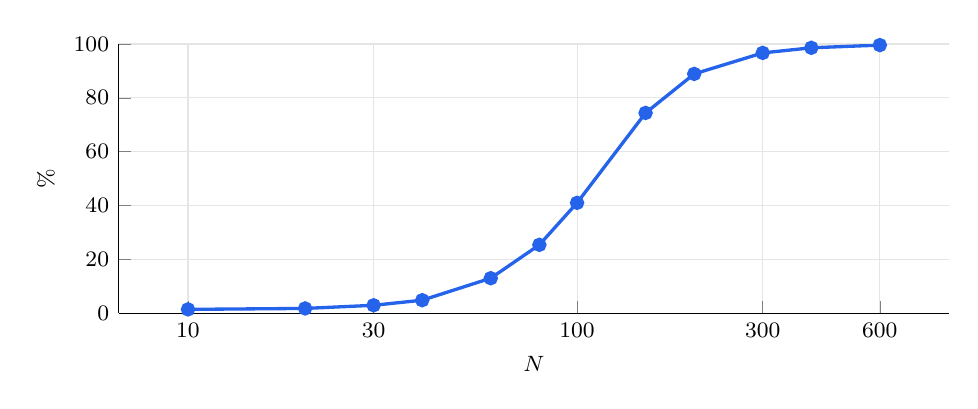
\begin{tikzpicture}
        \begin{axis}[
            width=\linewidth, height=5cm, xmode=log,
            xlabel={$N$}, ylabel={\%},
            xtick={10,30,100,300,600}, xticklabels={10,30,100,300,600},
            ymin=0, ymax=100]
          \addplot[cached,very thick,mark=*] coordinates {
            (10,1.42) (20,1.77) (30,2.94) (40,4.83) (60,13.0) (80,25.4) (100,41.0)
            (150,74.4) (200,88.9) (300,96.7) (400,98.6) (600,99.6)};
        \end{axis}
      \end{tikzpicture}
    \end{column}
  \end{columns}
  \vspace{0.3em}
  {\small The first use of each pair still runs the original arithmetic. At $N=100$
   only 41\,\% of operations are hits, so the gain is 1.3$\times$; from $N\approx600$
   more than 99\,\% are.}
\end{frame}

% ---------------------------------------------------------------------------
\begin{frame}{Peak memory before and after caching}
  \begin{columns}[c]
    \begin{column}{0.6\textwidth}
      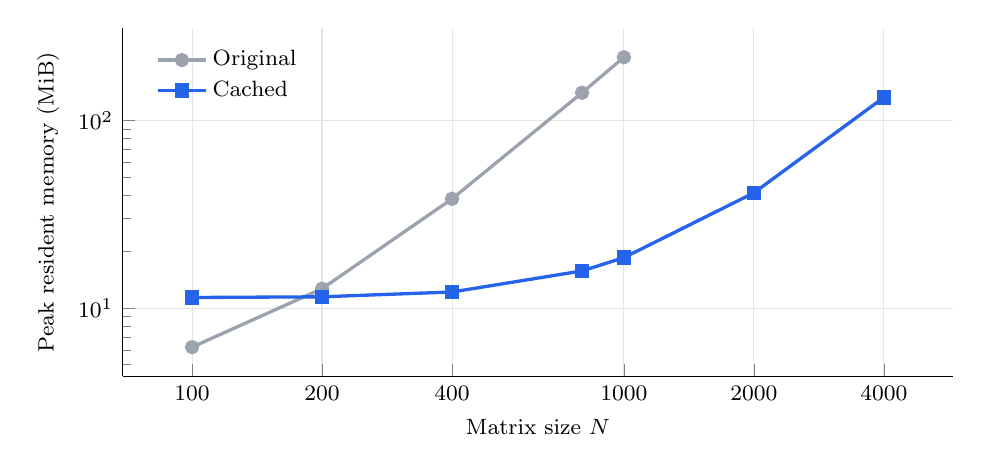
\begin{tikzpicture}
        \begin{axis}[
            width=\linewidth, height=6cm,
            xmode=log, ymode=log,
            xlabel={Matrix size $N$}, ylabel={Peak resident memory (MiB)},
            xtick={100,200,400,1000,2000,4000},
            xticklabels={100,200,400,1000,2000,4000},
            legend pos=north west]
          \addplot[original,very thick,mark=*] coordinates {
            (100,6.2) (200,12.7) (400,38.3) (800,140.8) (1000,217.7)};
          \addplot[cached,very thick,mark=square*] coordinates {
            (100,11.4) (200,11.5) (400,12.2) (800,15.8) (1000,18.6)
            (2000,41.2) (4000,133.0)};
          \legend{Original, Cached}
        \end{axis}
      \end{tikzpicture}
    \end{column}
    \begin{column}{0.37\textwidth}
      \stat{11.7$\times$ less}{at $N=1000$: 218 MiB $\rightarrow$ 18.6 MiB}
      \\[1em]
      \begin{itemize}\small
        \item An element shrinks from a heap-allocated polynomial
              ($\approx$ 56 bytes) to a 2-byte index.
        \item The tables cost a fixed $\approx$ 7 MB, so below $N=200$ the
              cached program uses \emph{more}.
      \end{itemize}
      {\scriptsize\color{muted}$N=4000$: 133 MiB here vs.\ 0.53 GB in the assignment text.}
    \end{column}
  \end{columns}
\end{frame}

% ---------------------------------------------------------------------------
\begin{frame}{Where the time goes after caching}
  \centering
  \begin{tabular}{@{}l r r r r@{}}
    \toprule
    Library & $N$ & Product (s) & Three determinants (s) & Product share \\
    \midrule
    Original & 1000 & 205   & 172 & 54\,\% \\
    Cached   & 4000 & 1\,053 & 128 & 89\,\% \\
    \bottomrule
  \end{tabular}
  \vspace{1.5em}
  \begin{itemize}
    \item After caching, the sequential $C = A\times B$ dominates the run time.
    \item The determinants are the part we distribute with MPI next.
  \end{itemize}
\end{frame}

% ---------------------------------------------------------------------------
\begin{frame}{MPI determinant: PLU with columns dealt out in panels}
  \begin{columns}[T]
    \begin{column}{0.5\textwidth}
      \begin{itemize}\small
        \item Gaussian elimination $PA = LU$; \;
              $\det A = (-1)^{\#\text{swaps}}\prod u_{kk}$.
        \item Exact arithmetic: \textbf{any nonzero} entry is a valid pivot,
              and no column is all zero unless $\det A = 0$.
        \item Panels of $b$ columns are dealt to the processes in turn
              (block-cyclic by column).
        \item The pivot and the multipliers of step $k$ are in column $k$, so the
              pivot search is \textbf{local}; row swaps need no messages.
      \end{itemize}
    \end{column}
    \begin{column}{0.47\textwidth}
      \begin{enumerate}\small
        \item[\textbf{1}] \textbf{Panel owner works alone.} Finds each pivot and the
              multipliers (via the field's reciprocal) in its own columns.
        \item[\textbf{2}] \textbf{One \texttt{MPI\_Bcast} per panel.} Singular flag,
              pivot rows and multipliers as raw 2-byte indices.
        \item[\textbf{3}] \textbf{Everyone updates its own columns.}
      \end{enumerate}
      \vspace{0.4em}
      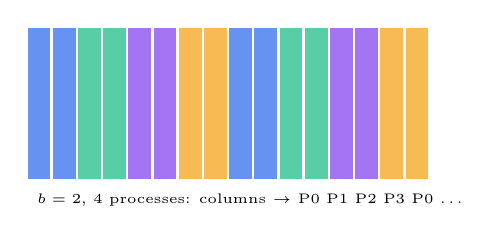
\begin{tikzpicture}[x=0.32cm,y=0.32cm]
        \foreach \c in {0,...,15} {
          \pgfmathtruncatemacro{\owner}{mod(floor(\c/2),4)}
          \ifcase\owner \def\col{cached}\or\def\col{ptwo}\or\def\col{pfour}\or\def\col{mapcol}\fi
          \fill[\col!70] (\c,0) rectangle (\c+0.9,6);
        }
        \node[font=\tiny,anchor=north west] at (0,-0.2)
          {$b=2$, 4 processes: columns $\to$ P0 P1 P2 P3 P0 \ldots};
      \end{tikzpicture}\\[0.3em]
      {\scriptsize Communication $\approx N^2$ bytes in total, one message per panel.}
    \end{column}
  \end{columns}
\end{frame}

% ---------------------------------------------------------------------------
\begin{frame}{Break-even: cached sequential vs.\ MPI}
  \begin{columns}[c]
    \begin{column}{0.6\textwidth}
      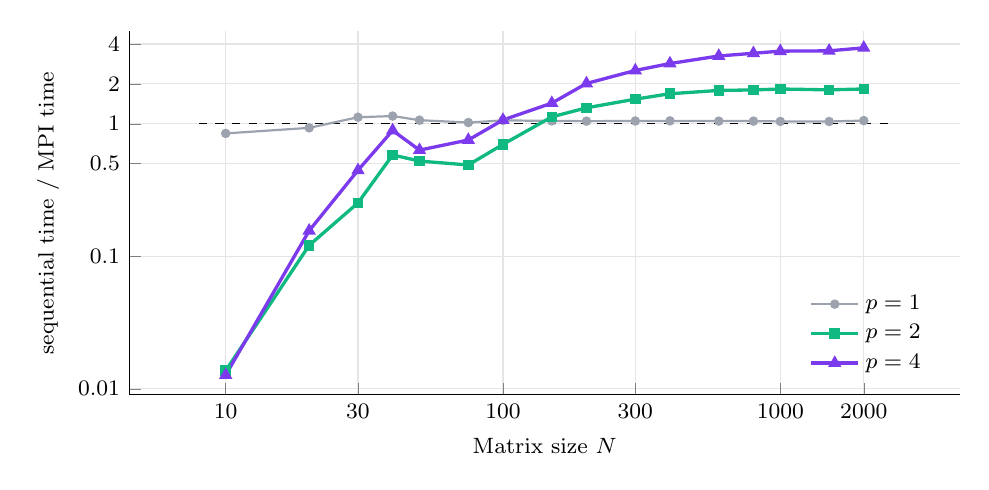
\begin{tikzpicture}
        \begin{axis}[
            width=\linewidth, height=6.2cm,
            xmode=log, ymode=log,
            xlabel={Matrix size $N$},
            ylabel={sequential time / MPI time},
            xtick={10,30,100,300,1000,2000},
            xticklabels={10,30,100,300,1000,2000},
            ytick={0.01,0.1,0.5,1,2,4},
            yticklabels={0.01,0.1,0.5,1,2,4},
            ymin=0.009, ymax=5,
            legend pos=south east]
          \addplot[domain=8:2500,samples=2,black,dashed,forget plot] {1};
          \addplot[original,thick,mark=*,mark size=1.3pt] coordinates {
            (10,0.846) (20,0.932) (30,1.121) (40,1.144) (50,1.065) (75,1.022)
            (100,1.061) (150,1.051) (200,1.047) (300,1.050) (400,1.052)
            (600,1.048) (800,1.048) (1000,1.042) (1500,1.041) (2000,1.057)};
          \addplot[ptwo,very thick,mark=square*,mark size=1.3pt] coordinates {
            (10,0.0137) (20,0.121) (30,0.253) (40,0.582) (50,0.523) (75,0.489)
            (100,0.700) (150,1.128) (200,1.320) (300,1.535) (400,1.686)
            (600,1.786) (800,1.802) (1000,1.831) (1500,1.804) (2000,1.832)};
          \addplot[pfour,very thick,mark=triangle*,mark size=1.6pt] coordinates {
            (10,0.0127) (20,0.156) (30,0.446) (40,0.891) (50,0.633) (75,0.755)
            (100,1.069) (150,1.433) (200,2.016) (300,2.527) (400,2.850)
            (600,3.250) (800,3.407) (1000,3.535) (1500,3.554) (2000,3.745)};
          \legend{$p=1$, $p=2$, $p=4$}
        \end{axis}
      \end{tikzpicture}
    \end{column}
    \begin{column}{0.37\textwidth}
      \small
      Cluster, $p$ processes on $p$ machines, $b=8$. Tested
      $N = 10,\ldots,2000$ (16 sizes).
      \begin{itemize}\small
        \item $p=4$: first faster at $N=100$, but only 1.07$\times$:
              within the noise. \textbf{Clearly faster from $N=150$} (1.43$\times$).
        \item $p=2$: faster from $N=150$.
        \item $N=2000$: 11.7 s $\rightarrow$ 3.2 s, \textbf{3.74$\times$} with 4 processes.
      \end{itemize}
      {\scriptsize\color{muted}$p=1$ is already $\approx$1.05$\times$ because its loop order
       differs from the sequential reference, not because of parallelism.}
    \end{column}
  \end{columns}
\end{frame}

% ---------------------------------------------------------------------------
\begin{frame}{Correctness of the MPI program}
  \begin{columns}[T]
    \begin{column}{0.5\textwidth}
      \begin{itemize}
        \item Every run also computes the cached sequential determinant on the
              \textbf{same matrices} (same seed and generator as \texttt{main.cpp})
              and exits with an error on a mismatch.
        \item All 1472 measured runs agreed.
      \end{itemize}
    \end{column}
    \begin{column}{0.46\textwidth}
      \stat{222 / 222}{test cases pass}
      \\[0.8em]
      {\small 1--4 processes; panel widths 1, 3, 16; awkward sizes 1, 2, 5, 17;
       matrices that force row swaps, zero multipliers, a zero leading entry or a
       zero determinant; and the values the original program prints.}
    \end{column}
  \end{columns}
\end{frame}

% ---------------------------------------------------------------------------
\begin{frame}{Limitations}
  \begin{columns}[T]
    \begin{column}{0.48\textwidth}
      \textbf{Measurements}
      \begin{itemize}\small
        \item Before/after timings come from one machine, 1--5 runs per size.
        \item The original library was not run beyond $N=1000$.
        \item Determinants under 0.1 s vary up to 2.2$\times$ between jobs;
              ratios near 1 mean little.
      \end{itemize}
    \end{column}
    \begin{column}{0.48\textwidth}
      \textbf{Design}
      \begin{itemize}\small
        \item The matrix product is still sequential.
        \item No look-ahead: other ranks wait while the next panel's owner factors it.
        \item Tables grow with $q^2$; fields larger than 4096 elements fall back to
              the original arithmetic.
        \item Each MPI process fills its own tables.
      \end{itemize}
    \end{column}
  \end{columns}
\end{frame}

% ---------------------------------------------------------------------------
\begin{frame}{Conclusions}
  \begin{columns}[T]
    \begin{column}{0.32\textwidth}
      \stat{24.7$\times$}{faster sequential program\\($N=1000$), 11.7$\times$ less memory}
    \end{column}
    \begin{column}{0.32\textwidth}
      \stat{1 entry}{in \texttt{Dependencies.cmake}; identical results on all 1\,771\,561 pairs}
    \end{column}
    \begin{column}{0.32\textwidth}
      \stat{3.74$\times$}{MPI determinant at $N=2000$, 4 machines; worth it from $N\approx150$}
    \end{column}
  \end{columns}
  \vspace{2em}
  \begin{itemize}
    \item Cache at the one class every operation passes through, and reuse its
          arithmetic on misses.
    \item Improve the sequential code first; then MPI pays off once the matrix
          is large enough to hide the broadcasts.
  \end{itemize}
\end{frame}

\begin{frame}[plain]
  \centering\vfill
  {\Huge\bfseries\color{accent} Questions?}\\[1em]
  {\small\color{muted}Code, measurements and report:
   \texttt{algebra-assignment} and \texttt{algebra-finite-fields-cached}}
  \vfill
\end{frame}

\end{document}
